\clearpage

\section{Компилятор графа вычислений}
\subsection{Граф вычислений}
\label{sec:compgraph}
\begin{figure}[ht]
    \centering
    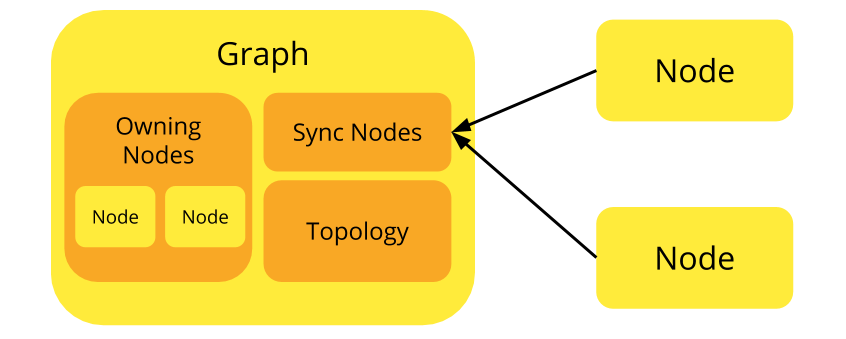
\includegraphics[width=0.8\linewidth]{graph.png}
    \caption{Граф вычислений}
    \label{fig:graphimpl}
\end{figure}
Граф представляет собой абстракцию, содержащую хранилище вершин графа с которыми работает пользователь в данный момент (Sync Nodes), сохраненные в графе вершины (Owning Nodes) и множество рёбер (Topology).
\begin{itemize}
    \item \textbf{Sync Nodes} -- хеш-таблица индексов вершин, объекты которых находятся у пользователя, и с которыми пользователь может работать (изменять, добавлять ассоциирующиеся с ними ребра в граф и т.п.).
    \item \textbf{Owning Nodes} - кортеж векторов вершин, сохраненных в графе, доступ к которым пользователь не имеет (заполняется при уничтожении вершины, ассоциируемой с графом, или после сохранения вершины пользователем).
    \item \textbf{Topology} - вектор, содержащий рёбра графа.
\end{itemize}
С помощью компилятора этот граф будет преобразован в последовательность машинных
команд, которые будут выполнены процессором. Но сперва необходимо выделить последовательность множеств вершин (назовем
их кластерами), работа с которыми может проводиться независимо внутри множеств. Кроме того вершинам i-го кластера требуются
данные только от вершин из предыдущих кластеров. Подобное разбиение позволит
с легкостью записать граф в виде обычной программы на некотором языке программирования,
а так же выполнить часть операций параллельно, эффективно задействуя многоядерные
системы.

Для выполнения такого разбиения разработан специальный алгоритм. На вход подаются
множество вершин графа, разделенное на вектора вершин соответствующих типов, с указанием количества входящих в каждую
вершину ребер и множество рёбер графа, представленное неотсортированным вектором.
Далее выполняются шаги:
\begin{enumerate}
    \item Отсортировать вектор рёбер. Назначить каждой вершине индекс, показывающий начало подвектора исходящих из неё рёбер.
    \item В множество вершин первого кластера заносятся все входные вершины графа. Их кластер назначается текущим.
    \item Пока из вершин текущего кластера есть выходящие ребра, повторяем:
    \begin{enumerate}
        \item Проходим по всем ребрам, выходящим из вершин текущего кластера и инкрементируем счетчик вхождений в иные вершины.
        \item Все иные вершины, счетчик соответствующий которым сравнялся с числом входящих в них на данной итерации рёбер кладем в новый кластер, назначаем его текущим и добавляем в последовательность. В случае если набрался лишь пустой кластер - новых элементов в последовательность не добавляем.
    \end{enumerate}
\end{enumerate}
\subsection{Генерация кода}
Как отмечалось ранее, в качестве основы для компилятора будет использоваться
фреймворк LLVM. Генерация кода производится с помощью следующего алгоритма
\begin{enumerate}
    \item Создать функцию \textit{jitmain}
    \item С помощью алгоритма, описанного в разделе \ref{sec:compgraph},
        генерируется структура обхода графа
    \item Для каждой вершины из обхода графа
        \begin{enumerate}
            \item Создать новую функцию для вычисления выходного значения
                вершины
            \item Если текущая вершина входная, то генерируется вызов метода
                аллокации памяти
            \item В противном случае для всех вершин, являющихся зависимостями
                текущей вершины генерируется вызов методов, блокирующих
                данные в памяти. Затем вызывается метод, который генерирует
                вызовы к соответствующим подпрограммам.
            \item Добавить вызов новой функции к телу \textit{jitmain}
            \item Для новой функции в ее \textit{метаданные} записывается
                информация о кластере, к которому принадлежит функция
        \end{enumerate}
    \item В зависимости от используемого оптимизатора генерируется необходимый
        код для обратного прохода.
\end{enumerate}

Функции, соответствующие вершинам графа, выполняют вызовы к библиотеке BLAS
(Basic Linear Algebra Subprograms) или другим вспомогательным математическим
подпрограммам. Последовательность этих вызовов определяется операцией, прикрепленной
к вершине. Аналогичным образом вычисляется производная.

Реализация этих методов находится в библиотеке среды выполнения. Это динамическая
библиотека, которую загружает \textit{драйвер} среды выполнения. В свою очередь,
драйвер -- статическая библиотека, содержащая объявления тех же методов, что и
библиотека среды выполнения, которой вызовы этих методов будут переданы.
В текущей реализации библиотека среды выполнения использует только CPU,
но в дальнейшем возможно расширение функционала за счет реализации других
библиотек.

Метаданные -- особая информация, которую LLVM добавляет инструкциям для
последующего использования при оптимизации и кодогенерации. Наиболее характерный
пример использования метаданных -- отладочная информация. Упомянутая в приведенном
выше алгоритме информация в последующем будет использоваться для автоматического
распараллеливания программы.

Результатом работы алгоритма станет LLVM IR, который будет подан на вход
JIT компилятору. В LLVM есть два способа выполнить JIT компиляцию: MCJIT
(Machine Code JIT) и ORC JIT (On Request Compiler JIT). Последний является
более современным и гибким решением. Концептуально схема компилятора
изображена на рис. \ref{fig:orcjit}. Сгенерированный LLVM IR сперва проходит
стадию оптимизации. На этом этапе к IR применяются различные оптимизации, в
частности автопараллелизация. Из полученного кода генерируются машинные инструкции.
В конце выполняется линковка получившейся программы с текущим процессом.

\begin{figure}[ht]
    \centering
    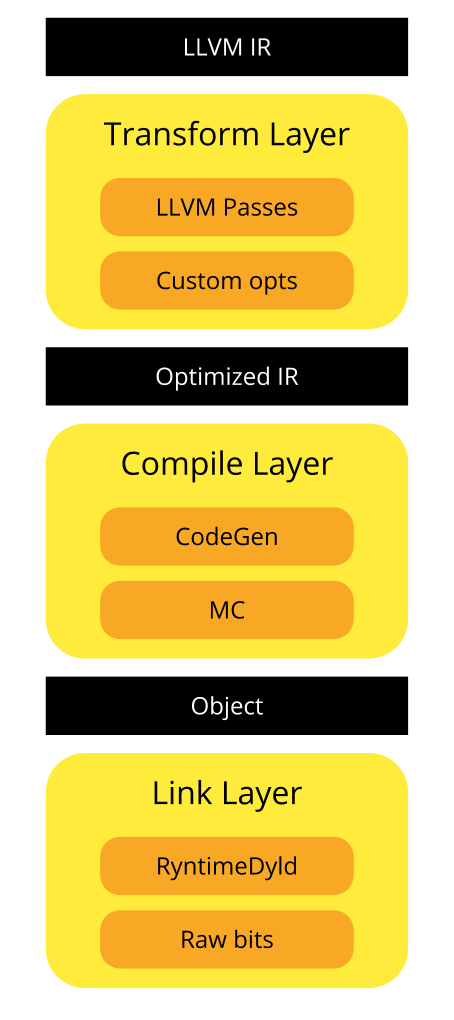
\includegraphics[width=0.4\textwidth]{orcjit.png}
    \caption{ORC JIT}
    \label{fig:orcjit}
\end{figure}
\subsection{Управление памятью}

Всем тензорам в графе присваивается уникальный номер -- виртуальный адрес.
С виртуальными адресами фреймворка можно выполнять те же операции, что и с
виртуальными адресами современных операционных систем: читать, писать, а так
же обращаться к памяти по какому-либо смещению. Во время исполнения графа
вычислений виртуальному адресу фреймворка ставится в соответствие виртуальный
адрес операционной системы. Такой подход обеспечивает гибкость и прозрачность
для пользователей фреймворка, но создает сложности для его разработчиков.
А именно:
\begin{enumerate}
    \item Как превратить виртуальный адрес фреймворка в адрес ОС?
    \item Как загрузить пользовательские данные в память?
\end{enumerate}

Для решения первой проблемы используется механизм аллокаторов. Аллокатор --
класс, реализующий методы allocate и deallocate, выделяющие и освобождающие
память соответственно. В рамках данной работы рассматривается так называемый
тривиальный аллокатор. Он ставит в соответствие тензору виртуальный адрес ОС.
Таким образом, для доступа к данным по некоторому смещению достаточно найти
тензор, для которого запрашиваемый адрес будет находиться в диапазоне [базовый адрес, базовый адрес + размер]
и выполнить аналогичные арифметические действия над виртуальным адресом ОС.

\begin{figure}[h]
    \centering
    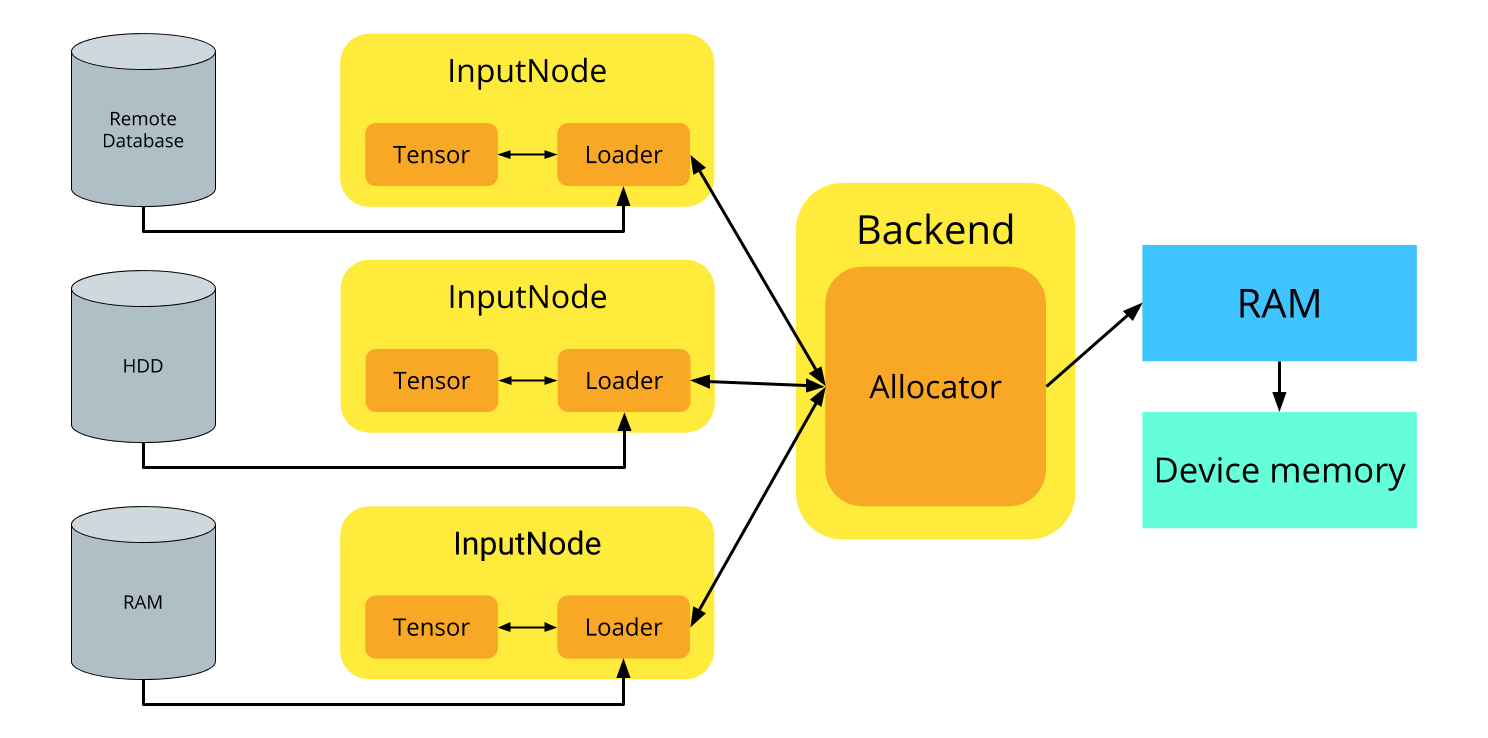
\includegraphics[width=0.8\linewidth]{loaders.png}
    \caption{Принципиальная схема работы загрузчика}
    \label{fig:loaders}
\end{figure}

Для решения второй проблемы предлагается ввести понятие загрузчика -- класса,
инкапсулирующего параметры, необходимые для доступа к данным. Такими параметрами
могут выступать имя базы данных и таблицы в ней, адрес в сети Интернет, путь
к локальному файлу, указатель на область оперативной памяти. Схематично
работа загрузчиков описана на рис. \ref{fig:loaders}.
В ядре фреймворка присутствует класс Loader, являющийся абстрактным загрузчиком.
Для него определены виртуальные методы:
\begin{itemize}
    \item \texttt{void load(athena::core::Allocator *)} -- выполняет непосредственную загрузку данных в RAM
    \item \texttt{std::string getLoadCName()} -- возвращает имя функции-обертки загрузки для данной реализации загрузчика
    \item \texttt{std::string getCreateCName()} -- возвращает имя функции-обертки создания для данной реализации загрузчика
    \item \texttt{serialize()} -- сериализует объект для сохранения в файле
\end{itemize}
Реализации имеют специальные C-style методы. Их назначение заключается в
создании интерфейса для доступа из автоматически сгенерированного кода.
\begin{lstlisting}
extern "C" {
<loaderName>Load(athena::core::Allocator*, Loader* loader) // load wrapper
<loaderName>Create(/* ctor args */) // c-tor wrapper
}
\end{lstlisting}

\subsection{Отладка и профилирование}

Поскольку для каждой вершины генерируется собственная функция, у пользователя
появляется возможность точечно влиять на исполнение графа. А именно, выполнять
отладку и профилирование нейронной сети.

Отладчик имеет клиент-серверную архитектуру. Сервер встраивается непосредственно
в фреймворк. Во время генерации кода к функциям, соответствующим вершинам
добавляются вызовы к методам серверной части отладчика. Таким образом можно реализовать
точки останова. Достаточно в вызываемой функции захватить мьютекс.

Клиентская часть -- отдельная программа, которая общается с сервером через сокет.
Она запрашивает граф в сериализованном виде и передает серверу информацию об
установленных точках останова. Пользователь может запросить данные из некоторого
тензора. Клиент получит их, обработает и представит в графическом виде.

\begin{figure}[ht]
    \centering
    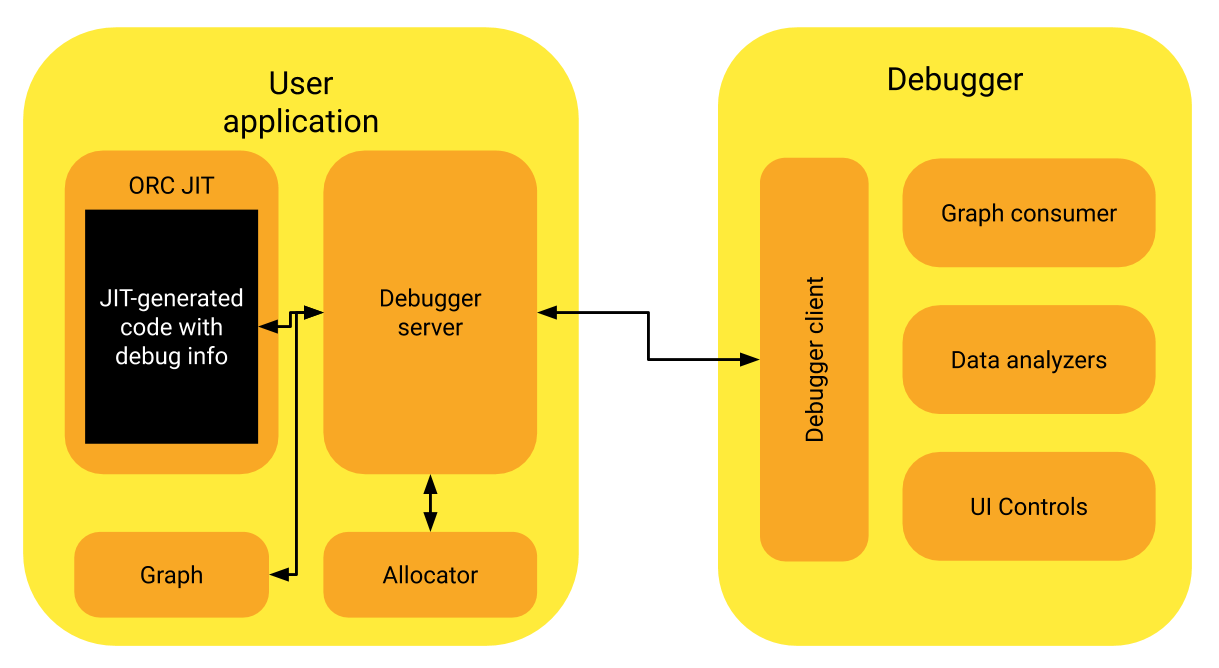
\includegraphics[width=0.8\linewidth]{debugger.png}
    \caption{Принципиальная схема работы отладчика}
    \label{fig:debugger}
\end{figure}

